\chapter{Cơ sở lý thuyết}
\section{Giới thiệu về Turtlebot3}
\subsection{TurtleBot3 là gì?}
\tab TurtleBot3 là một robot nhỏ gọn có thể lập trình trên nền tảng ROS với mức chi phí thấp. Nó được thiết kế để sử dụng trong giáo dục, nghiên cứu, sở thích hoặc là muốn tạo ra một sản phẩm mới. TurtleBot3 là một dòng robot thế hệ mới được thiết kế dưới dạng modular, nhỏ gọn và hoàn toàn có thể tùy biến theo cá nhân. Ngoài ra, do được sử dụng rộng rãi, TurtleBot3 có cộng đồng hỗ trợ và các bài viết học thuật hỗ trợ kết nối và sử dụng phần cứng.
\subsection{Đặc điểm}
\begin{enumerate}
    \item \textit{Kiểu dáng nhỏ gọn:} TurtleBot3 có kiểu dáng nhỏ gọn, giúp nó dễ dàng di chuyển trong các môi trường có không gian hạn chế.
    \item \textit{Hệ thống chuyển động}: Với bốn bánh xe đa hình, TurtleBot3 có khả năng di chuyển một cách linh hoạt và chính xác, phù hợp cho nhiều ứng dụng trong nghiên cứu và giáo dục.
    \item \textit{Sử dụng ROS\textsuperscript{\cite{ros}} (Robot Operating System)}: TurtleBot3 tích hợp chặt chẽ với ROS, một hệ thống mã nguồn mở cho robot, giúp tạo môi trường phát triển và thử nghiệm linh hoạt.
    \item \textit{Dòng robot đa dạng:} TurtleBot3 có các mô hình robot như Burger và Waffle, với các tính năng và hiệu suất phù hợp với nhu cầu sử dụng cụ thể.   
    \begin{figure}[htp]
        \begin{subfigure}{0.5\textwidth}
        \centering
        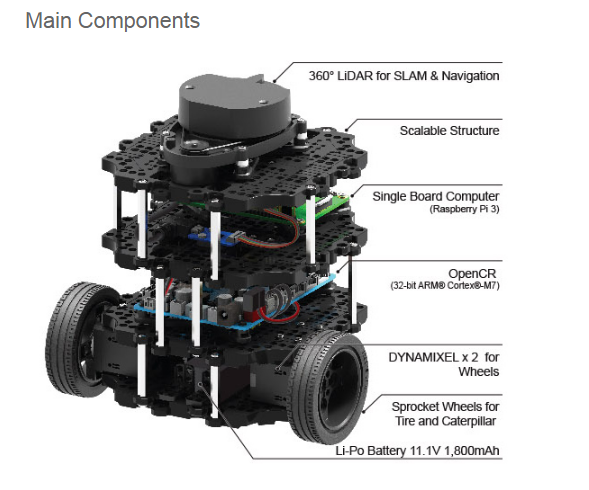
\includegraphics[width=7cm]{img/2_Theory/turtlebot3_burger.png}
        \caption{TurtleBot3 Burger}
        \end{subfigure}%
        \begin{subfigure}{0.5\textwidth}
        \centering
        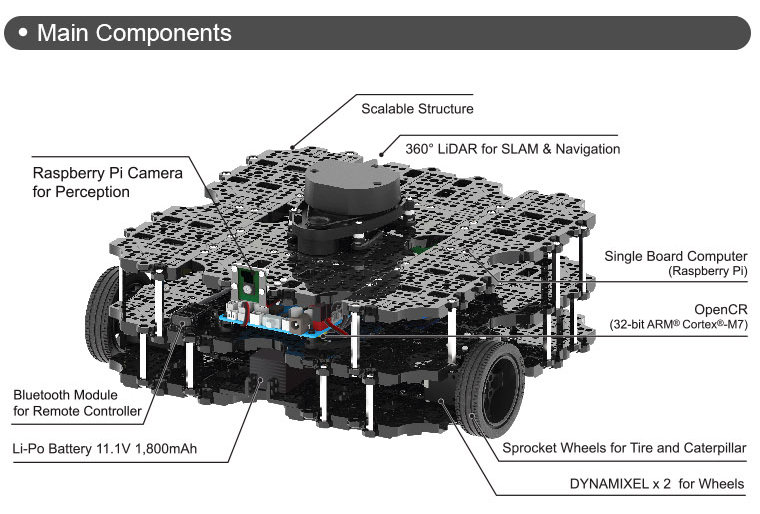
\includegraphics[width=7cm]{img/2_Theory/turtlebot3_waffle_pi.jpg}
        \caption{TurtleBot3 Waffle}
        \end{subfigure}
    \caption{Các dòng robot của TurtleBot3}
    \end{figure}
    \item \textit{Cảm biến}: Được trang bị với các cảm biến như cảm biến hồng ngoại, bộ cảm biến IMU (Inertial Measurement Unit), và camera, TurtleBot3 có khả năng thu thập dữ liệu môi trường và chính xác hóa động tác.
    \item \textit{Môi trường mô phỏng Gazebo:} TurtleBot3 được tích hợp chặt chẽ với Gazebo, một môi trường mô phỏng 3D, giúp người dùng kiểm thử và phát triển ứng dụng trong môi trường an toàn trước khi triển khai trên robot thực tế.
    \item \textit{Hỗ trợ học máy và trí tuệ nhân tạo:} Với tích hợp chặt chẽ với ROS, TurtleBot3 có thể được sử dụng để triển khai các thuật toán và mô hình học máy, từ điều hướng tự động đến nhận diện vật thể.
    \item \textit{Cộng đồng lớn và nguồn mở:} TurtleBot3 là một dự án nguồn mở với sự đóng góp từ cộng đồng lớn, tạo điều kiện cho việc chia sẻ kiến thức và phát triển cộng đồng người dùng.
\end{enumerate}
\subsection{Bài toán và ứng dụng đặt ra cho TurtleBot3}
\begin{itemize}
    \item \textit{Bài toán tránh vật cản:} Robot phải có khả năng phát hiện và tránh các vật cản trên đường đi của nó, bằng cách sử dụng các cảm biến và thuật toán học sâu.
    \item \textit{Bài toán điều hướng:} Robot phải có khả năng xác định vị trí của mình trong môi trường, bằng cách sử dụng các phương pháp như SLAM (Simultaneous Localization and Mapping) hoặc GPS (Global Positioning System).
    \item \textit{Bài toán giao tiếp:} Robot phải có khả năng giao tiếp với con người hoặc các robot khác, bằng cách sử dụng các phương tiện như âm thanh, hình ảnh, cử chỉ hoặc mạng không dây.
    \item \textit{Bài toán hợp tác:} Robot phải có khả năng hợp tác với các robot khác để thực hiện một nhiệm vụ chung, bằng cách sử dụng các thuật toán phối hợp và phân công.
\end{itemize}
\subsection{TurtleBot và phần cứng đã trang bị}
\begin{itemize}
    \item \textit{Robot:} Để phù hợp với làn đường, nhóm đã chọn Turtlebot dạng Burger. Bởi Burger cho phép ta đặt camera ở góc nhìn cao hơn, giống với thực tế hơn
    \item \textit{Camera:} Để có tầm nhìn bao quát cả phần dưới robot, nhóm đã trang bị camera với trường nhìn (FOV) là 160 độ
\end{itemize}
\section{ROS}
\subsection{ROS là gì?}
\begin{figure}[htp]
\begin{center}
    \includegraphics[width=7cm]{img/2_Theory/ROS.png}
    \caption{Logo ROS}
\end{center}
\end{figure}
\hspace{0.4cm}ROS\textsuperscript{\cite{ros}}, viết tắt của "Robot Operating System" (Hệ điều hành Robot), là một framework mã nguồn mở được thiết kế để hỗ trợ việc phát triển phần mềm cho robot. ROS không phải là hệ điều hành robot như tên gọi có thể khiến người ta hiểu lầm, mà nó là một tập hợp các công cụ, thư viện, và quy tắc chuẩn hóa giúp đơn giản hóa quá trình phát triển và chia sẻ phần mềm giữa các dự án robot.\\
\tab ROS được phát triển chủ yếu bởi Willow Garage và hiện nay được duy trì và phát triển bởi Open Robotics. Nó cung cấp một loạt các tính năng như quản lý thiết bị phần cứng, truyền thông giữa các module, quản lý gói phần mềm, và nhiều công cụ hỗ trợ khác để giúp nhà phát triển robot xây dựng và kiểm thử phần mềm của họ một cách dễ dàng.\\
\tab ROS là một hệ thống phần mềm phổ biến trong cộng đồng nghiên cứu và phát triển robot, được sử dụng rộng rãi trong các dự án về robot tự hành, robot công nghiệp, và nhiều ứng dụng khác liên quan đến lĩnh vực robotics.
\subsection{Ưu điểm của ROS}
\begin{enumerate}
    \item \textit{Mã nguồn mở, hoàn toàn miễn phí:} ROS là một dự án mã nguồn mở, điều này có nghĩa là người dùng có thể truy cập hoàn toàn miễn phí và sửa đổi mã nguồn theo nhu cầu.
    \item \textit{Tính linh hoạt:} ROS hỗ trợ nhiều ngôn ngữ lập trình như C++, Python,... giúp người phát triển lựa chọn ngôn ngữ phù hợp với kỹ năng và yêu cầu của dự án. (Source code của nhóm sử dụng ngôn ngữ Python để lập trình.)
    \item \textit{Thư viện và công cụ mạnh mẽ:}
    \begin{itemize}
        \item ROS cung cấp nhiều thư viện và công cụ hỗ trợ như thư viện điều khiển robot, thư viện thị giác máy tính, công cụ giả lập, và nhiều công cụ khác.
        \item Gazebo, một môi trường mô phỏng tích hợp sâu với ROS, giúp người phát triển kiểm thử và mô phỏng robot một cách hiệu quả.
    \end{itemize}
\end{enumerate}
\subsection{Phiên bản sử dụng}
\tab Hiện nay có khá nhiều phiên bản ROS như là ROS Kinetic, ROS Melodic, ROS Dashing,... Đối với đồ án này, nhóm quyết định sử dụng ROS Noetic. ROS Noetic là phiên bản thứ 13 của ROS. Nó được phát hành vào ngày 23 tháng 5 năm 2020. ROS Noetic chủ yếu hướng tới Ubuntu 20.04 (Focal), mặc dù các hệ thống khác được hỗ trợ ở các mức độ khác nhau.
\subsection{Các topic sử dụng}
\subsubsection{camera/image/compressed}
\subsubsection{cmd\_vel}
Ngoài các topic có sẵn của turtlebot ra, nhóm còn tạo các topic minh hoạ dữ liệu của các module để thuận tiện trong quá trình sửa lỗi.
\section{Gazebo}
\subsection{Gazebo là gì?}
\begin{figure}[h]
\begin{center}

\includegraphics[width=8cm]{img/2_Theory/gazebo.png}
\caption{Logo Gazebo}
\end{center}
\end{figure}
\hspace{0.4cm}Gazebo\textsuperscript{\cite{gazebo}} là một môi trường mô phỏng 3D mã nguồn mở được sử dụng chủ yếu trong lĩnh vực nghiên cứu và phát triển robot. Nó cung cấp một không gian ảo cho việc thử nghiệm, kiểm thử, và phát triển ứng dụng robot mà không cần phải triển khai trên robot thực tế.
\subsection{Đặc điểm}
\begin{enumerate}
    \item \textit{Mô phỏng chính xác:} Gazebo cung cấp một môi trường mô phỏng chính xác với độ chi tiết cao, giúp người phát triển kiểm thử và đánh giá hiệu suất của ứng dụng robot mà không cần phải thực hiện trên thiết bị thực tế.
    \item \textit{Đa nền tảng:} Hỗ trợ trên nhiều hệ điều hành như Linux, macOS, và Windows.
    \item \textit{Hỗ trợ công nghệ ROS:} Gazebo tích hợp chặt chẽ với ROS, giúp dễ dàng tích hợp và kiểm thử các ứng dụng ROS trong môi trường mô phỏng.
    \item \textit{Tích hợp với công cụ phát triển:} Gazebo tích hợp với các công cụ phát triển như RViz\textsuperscript{\cite{rviz}} và RQT, tạo ra một môi trường phát triển toàn diện cho robot.
    \item \textit{GUI (Graphical User Interface):} Gazebo cung cấp GUI thân thiện, dễ sử dụng với người dùng, thông qua các thanh menu, giúp người dùng tương tác trực tiếp trên gazebo mà không cần thông qua chỉnh sửa tệp mã.
\end{enumerate}
\subsection{Phiên bản sử dụng}
\tab Như đã giới thiệu ở phần \textbf{Đặc điểm}, Gazebo được tích hợp chặt chẽ với ROS, và ROS lại tương thích tốt với Ubuntu, nên nhóm đã cài đặt và sử dụng Gazebo phiên bản 11.11.0 trên Ubuntu để tiện cho việc mô phỏng.
\subsection{Mô tả robot}
\tab Để mô phỏng robot trong Gazebo, ta cần mô tả nó trong trong một file URDF (Unified Robot Description Format). URDF về cơ bản là một tệp XML cho phép mô tả các thuộc tính vật lý quan trọng của rô-bốt chẳng hạn như link (liên kết), joint (khớp nối), hình dạng, màu sắc, collision (va chạm), v.v. Trong đó tất cả các thành phần (liên kết và khớp nối) được định nghĩa bằng cách sử dụng tag.  Phiên bản URDF của Turtlebot3 Burger được nhóm lấy từ package Turtlebot3 Autorace 2020\textsuperscript{\cite{autorace}}.
\begin{figure}[!htb]
\begin{center}
    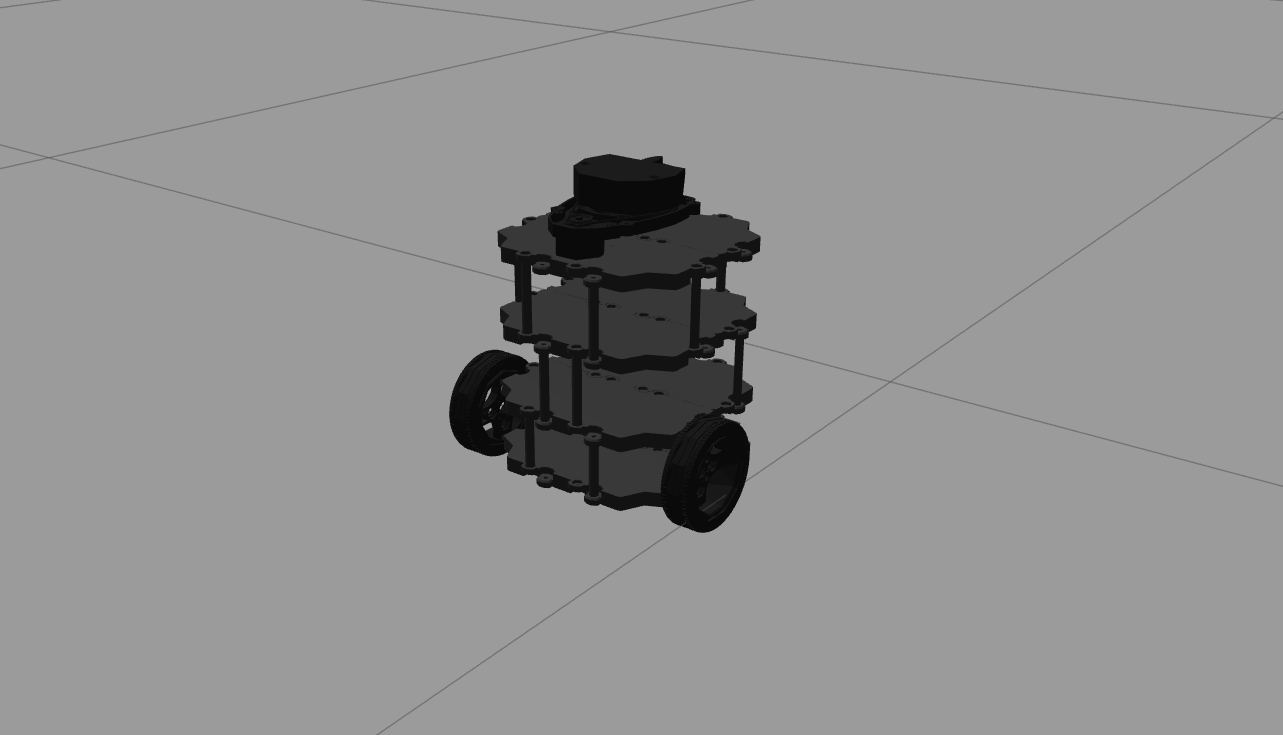
\includegraphics[width=12cm]{img/2_Theory/turtlebot3_burger_gazebo.png}
    \caption{Turtlebot3 Burger trong Gazebo}
\end{center}
\end{figure}
\subsection{Model làn đường}
\tab Gazebo sử dụng SDF (Simulation Description Format) để mô tả các yếu tố khác nhau của vật thể như robot, cảm biến, đèn, và các đối tượng môi trường như đất, tường, hoặc các vật thể khác. Nó giúp xác định vị trí, hình dạng, và các thuộc tính khác của các phần tử trong môi trường 3D.\\
\tab Phần mềm mà nhóm sử dụng để thiết kế model trong Gazebo là Blender\textsuperscript{\cite{blender}}. Blender là một phần mềm đồ họa 3D mã nguồn mở, mạnh mẽ và linh hoạt, phục vụ nhu cầu của nhiều lĩnh vực như đồ họa máy tính, nghệ thuật số, mô phỏng, và phát triển trò chơi.
\begin{figure}[!htb]
\begin{center}
    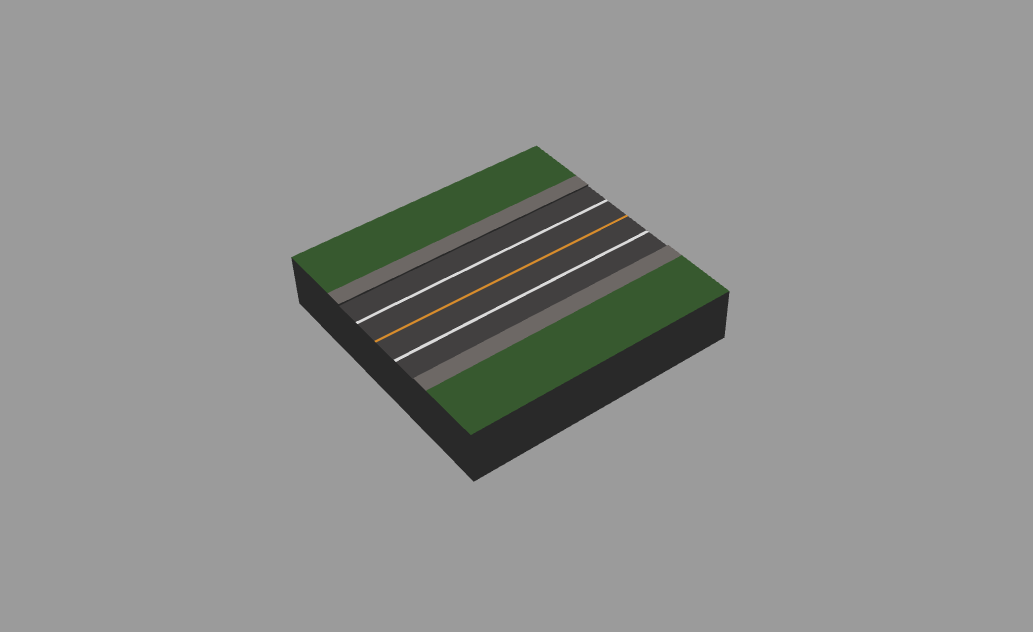
\includegraphics[width=12cm]{img/2_Theory/lane_model.png}
    \caption{Một phần làn đường trong Gazebo}
\end{center}
\end{figure}
\newpage
\section{Unity}
Ngoài công cụ mô phỏng Gazebo ra, nhóm còn sử dụng Unity để tạo dữ liệu cho việc huấn luyện model. Unity là Game Engine
\newpage
\section{OpenCV}
\subsection{OpenCV là gì?}
\begin{figure}[!hbt]
\begin{center}
    
\includegraphics[width=4cm]{img/2_Theory/opencv.png}
    \caption{Logo OpenCV}
\end{center}
\end{figure}
\tab OpenCV\textsuperscript{\cite{opencv}}, hay Open Source Computer Vision Library, là một thư viện mã nguồn mở chuyên về thị giác máy tính và xử lý ảnh. OpenCV được thiết kế để cung cấp một loạt các công cụ và thuật toán tiện ích để xử lý ảnh và video. Đồng thời, nó cũng được thiết kế để hỗ trợ hiệu quả về tính toán và chuyên dùng cho các ứng dụng thời gian thực. OpenCV có các giao diện cho ngôn ngữ lập trình C++, C, Python và Java và hỗ trợ các hệ điều hành như Windows, Linux, Mac OS, iOS và Android. 
\subsection{Ứng dụng}
\tab OpenCV được sử dụng cho đa dạng nhiều mục đích và ứng dụng khác nhau bao gồm: 
\begin{itemize}
    \item Hình ảnh street view.
    \item Kiểm tra và giám sát tự động.
    \item Robot và xe hơi tự lái.
    \item Phân tích hình ảnh y học.
    \item Tìm kiếm và phục hồi hình ảnh/video.
    \item Phim – cấu trúc 3D từ chuyển động.
    \item Nghệ thuật sắp đặt tương tác.
\end{itemize}
\subsection{Tính năng}
\begin{enumerate}
    \item \textit{Xử lý ảnh và video:} OpenCV cung cấp các thuật toán và công cụ để xử lý ảnh và video, bao gồm lọc ảnh, biến đổi hình thái, phát hiện cạnh, và nhiều công cụ khác.
    \item \textit{Thị giác máy tính:} Thư viện này hỗ trợ nhiều thuật toán thị giác máy tính, bao gồm nhận diện khuôn mặt, nhận diện đối tượng, theo dõi đối tượng, và nhận diện ký tự.
    \item \textit{Machine learning:} OpenCV tích hợp với các thư viện máy học như TensorFlow và PyTorch để thực hiện các nhiệm vụ như học máy và học sâu.
    \item \textit{Xử lý ảnh y tế: }OpenCV được sử dụng trong lĩnh vực y tế để phân tích hình ảnh y khoa và hỗ trợ các ứng dụng như dự đoán bệnh, phân loại tế bào, và nhiều công việc khác.
    \item \textit{Robotics:} OpenCV được tích hợp trong nhiều dự án robotics để xử lý ảnh từ các camera và cảm biến.
    \item \textit{Real-time Computer Vision:} OpenCV hỗ trợ thị giác máy tính thời gian thực, làm cho nó phù hợp cho ứng dụng như xe tự lái, video giám sát, và robot di động.
\end{enumerate}
\subsection{Chọn ngôn ngữ nào để lập trình OpenCV?}
\tab OpenCV hiện tại hỗ trợ nhiều ngôn ngữ, mỗi ngôn ngữ có thế mạnh riêng, vậy thì tùy theo nhu cầu mà chọn ngôn ngữ cho phù hợp.
\begin{itemize}
    \item \textit{C++:} Đây là ngôn ngữ phổ biến nhất hiện tại vì nhanh, có nhiều lựa chọn.
    \item \textit{Python:} Ngôn ngữ được dùng nhiều để thử nghiệm/kiểm tra OpenCV do tính ngắn gọn, ít phải thiết lập. Bên cạnh đó, nếu dùng Python thì cũng có thể code được trên nhiều hệ điều hành.
    \item \textit{Java:} Nhanh và đa nền tảng, tương tự C++.
\end{itemize}
\tab Đối với đề tài, nhóm sử dụng ngôn ngữ Python để lập trình.
\section{Thuật toán Hough Line Transform}
\subsection{Phương trình đường thẳng trong không gian ảnh}
\tab Ở cấp bậc trung học, chúng ta đã biết phương trình đường thẳng cơ bản được biểu diễn bởi 2 tham số $a$ và $b$ như sau:
\begin{center}
$y = ax + b$    
\end{center}
\begin{figure}[htp]
\begin{center}
    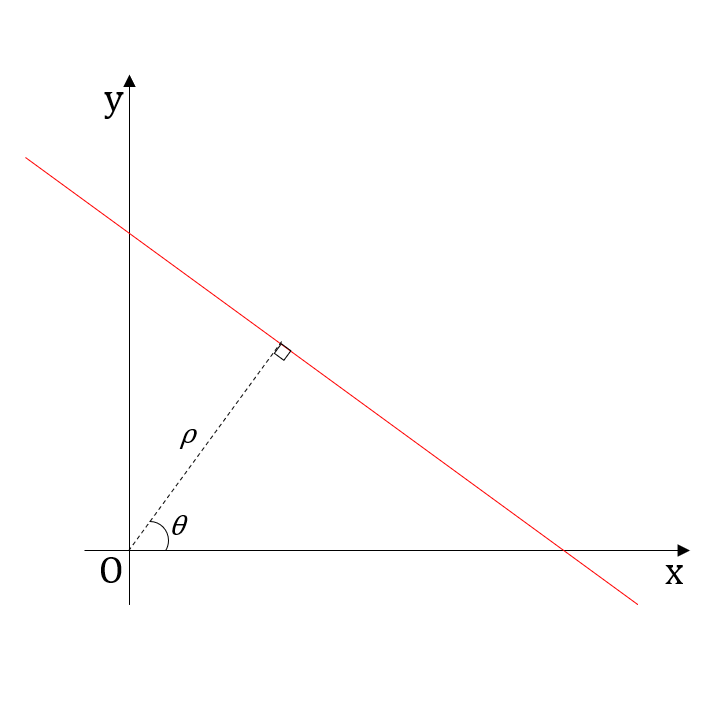
\includegraphics[width=8cm]{img/2_Theory/hough_trans_1.png}
    \caption{Phương trình đường thẳng $y = ax + b$ trong không gian ảnh}
\end{center}
\end{figure}
\tab Tuy nhiên, với cách biểu diễn này, giá trị của hệ số chặn $a$ trải dài từ $-\infty$ đến $+\infty$. Có thể lấy ví dụ, để có được phương trình đường Oy $(x = 0)$ thì $a$ phải tiến tới $\infty$. Thuật toán Hough  Line Transform\textsuperscript{\cite{houghtransform}} yêu cầu các giá trị $a$, $b$ nằm trong một khoảng xác định (hay bị chặn trên dưới), ta phải sử dụng hệ tọa độ cực để biểu diễn phương trình đường thẳng. Cách biểu diễn này cũng nằm trong chương trình toán trung học:
\begin{center}
$\rho = xcos(\theta) + ysin(\theta)$    
\end{center}
với $\rho$ là khoảng cách vuông góc từ gốc tọa độ O tới đường thẳng và $\theta$ là góc hợp bởi đường thẳng vuông góc này với trục hoành, được tính theo ngược chiều kim đồng hồ.\\
\tab Xét thấy trong phương trình tọa độ cực, giá trị của góc $\theta$ có thể bị chặn lại trong khoảng $[0, \pi)$. Trên thực tế, không gian ảnh là không gian hữu hạn (bị chặn lại bởi các cạnh của ảnh), do vậy giá trị $\rho$ cũng bị chặn.
\subsection{Ánh xạ giữa không gian ảnh và không gian Hough}
\tab Từ một đường thẳng trong không gian ảnh với 2 tham số là $\rho$ và $\theta$, ta sẽ ánh xạ sang không gian Hough thành 1 điểm.
\begin{figure}[htp]
\begin{center}
    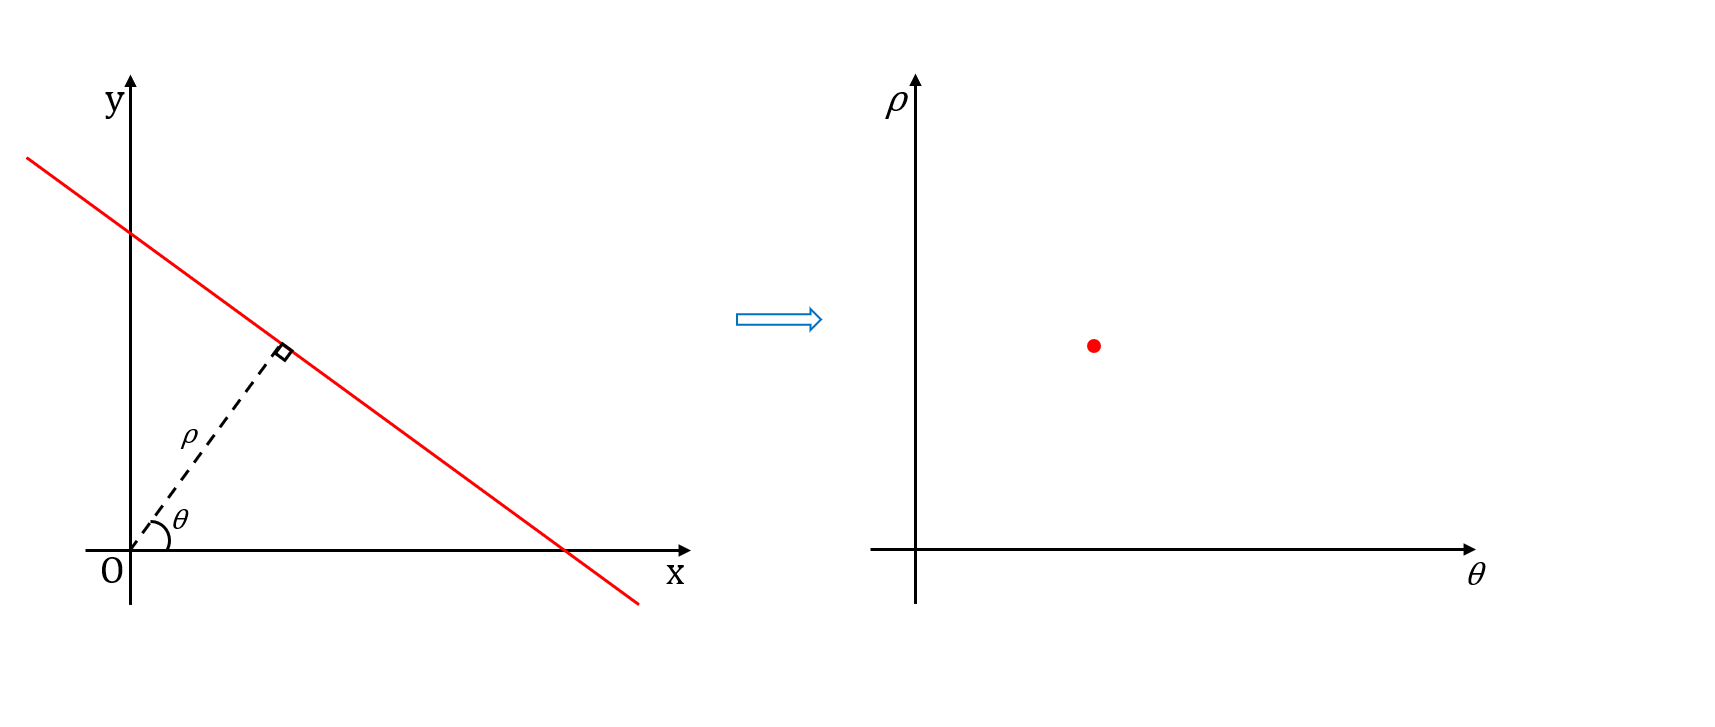
\includegraphics[width=13cm]{img/2_Theory/hough_trans_3.jpg.png}
    \caption{\centering Ánh xạ một đường thẳng từ không gian ảnh thành một điểm trong không gian Hough}
\end{center}
\end{figure}
\newpage
\tab Còn từ một điểm trong không gian ảnh, có tọa độ $(x, y)$, ta thu được một hình sin trong không gian Hough.\\
\begin{figure}[!htp]
\begin{center}
    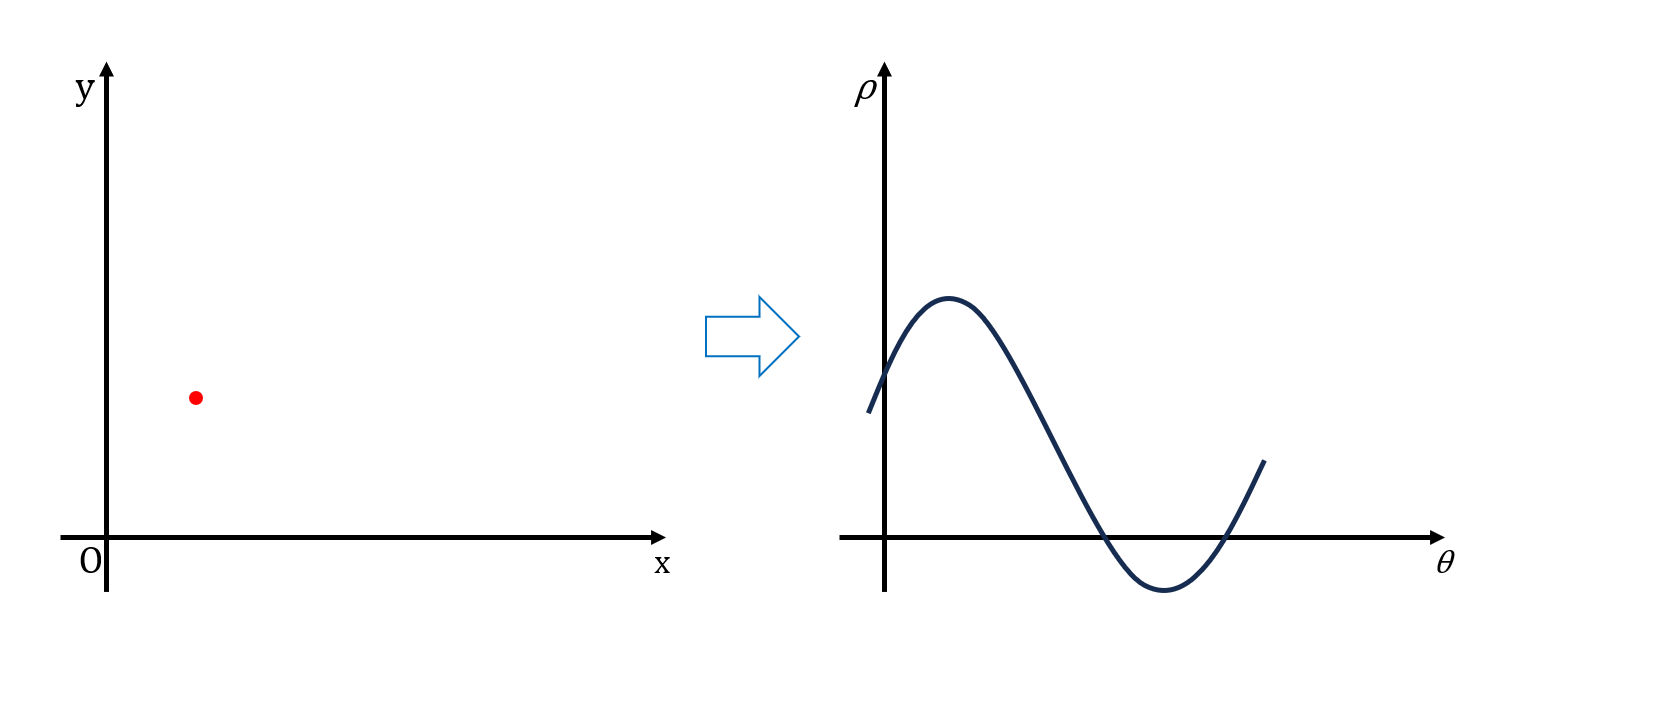
\includegraphics[width=12cm]{img/2_Theory/hough_trans_4.jpg.png}
    \caption{\centering Ánh xạ một điểm từ không gian ảnh thành một hình sin trong không gian Hough}
\end{center}
\end{figure}
\\
\tab Các điểm nằm trên cùng một đường thẳng sẽ biểu diễn được các hình sin giao nhau tại một điểm trong không gian Hough. Dựa vào ý tưởng này, thuật toán Hough Line Transform sẽ chọn được phương trình đường thẳng đi qua nhiều điểm nhất thông qua việc bình chọn. Tuy nhiên, trong thực tế, trong một bức ảnh thường có nhiều hơn một cạnh, như vậy, việc lấy đường thẳng có số pixel đi qua nhiều nhất sẽ không phù hợp. Thay vào đó, chúng ta sẽ đặt ra một ngưỡng số lượng pixel nhất định, nếu trên ngưỡng này thì được xem là đường thẳng và ngược lại.
\begin{figure}[htp]
\begin{center}
    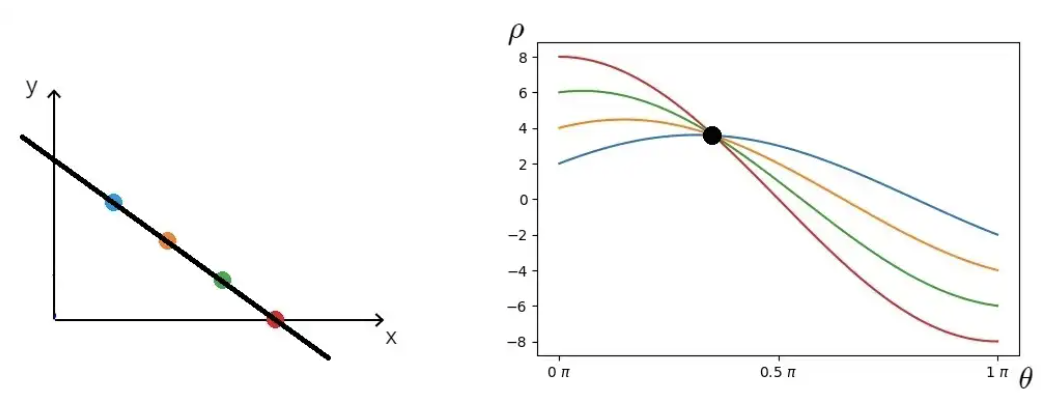
\includegraphics[width=14cm]{img/2_Theory/hough_trans_5.png}
    \caption{\centering Hình ảnh minh họa cho ánh xạ nhiều điểm trên đường thẳng trong không gian ảnh sang không gian Hough}
\end{center}
\end{figure}
\subsection{Hough Line Transform hoạt động như thế nào?}
\subsubsection{Tiền xử lý}
\tab Để thu được các đường thẳng như mong muốn, ảnh cần được xử lý trước khi thực hiện thuật toán Hough Line Transform. Hough Line Transform yêu cầu đầu vào là một ảnh nhị phân. Trên thực tế ảnh sẽ được đưa về dạng ảnh xám, áp dụng các thuật toán lọc biên để xác định các đường biên trong ảnh. Ở đây chúng ta sẽ sử dụng thuật toán Canny để lọc biên. \\
\tab Đối với đề tài của nhóm, đầu vào của thuật toán Hough Line Transform là một ảnh dạng nhị phân, do đó ta sẽ bỏ qua bước tiền xử lý này.
\subsubsection{Bình chọn đường thẳng}
\tab Ta chia không gian Hough thành các lưới ô vuông nhỏ. Ta thu được một lưới ô vuông (ma trận) với các hàng là trục $\rho$ và các cột là trục $\theta$ như hình \ref{accumlator}. Độ chính xác của thuật toán phụ thuộc vào số lượng các ô vuông ta chọn cho mỗi cạnh. Giả sử ta muốn độ chính xác của $\theta$ là $1^{\circ}$, ta cần 180 cột. Giá trị $\rho$ bị chặn bởi cạnh chéo của ảnh đầu vào. Do vậy khi lấy độ chính xác của $\rho$ là 1 (pixel) thì số hàng bằng độ dài đường chéo ảnh theo đơn vị pixel.\\
\begin{figure}[ht]
\begin{center}
    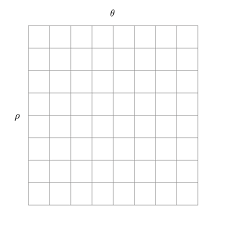
\includegraphics[width=6cm]{img/2_Theory/hough_trans_2.png}
    \caption{Lưới ô vuông (ma trận) minh họa thu được từ không gian Hough}
    \label{accumlator}
\end{center}
\end{figure}
\newpage
\tab Giá trị tại mỗi ô ban đầu trong ma trận được đặt bằng 0. Xét các điểm trên ảnh đầu vào (chính là ảnh nhị phân thu được sau bước tiền xử lý), với mỗi điểm sáng, ta xét $\theta$ trong khoảng $[0, 180)$. Vì đã biết tọa độ điểm $(x, y)$, ta dễ dàng tính được giá trị $\rho$. Với mỗi cặp ($\rho, \theta$), ta thực hiện bình chọn (tăng giá trị ô tương ứng trong ma trận lên 1 đơn vị). Cuối cùng ta thực hiện lấy ngưỡng để xác định trên lưới ô vuông đường thẳng nào ứng với một đường thẳng trên thực tế.
\section{K-means Clustering}
\section{Curve fitting}
\section{Image Segmentation}
\subsection{Image Segmentation là gì}
\tab Image Segmentation (phân đoạn ảnh) là một phần quan trọng trong lĩnh vực Computer Vision (thị giác máy tính). Nó là quá trình chia nhỏ một bức ảnh thành nhiều phần, với mục tiêu đơn giản hóa hoặc thay đổi biểu diễn của bức ảnh để dễ dàng phân tích. Image Segmentation cũng có một mục tiêu chung với Object Detection (phát hiện vật thể) là phát hiện ra vùng ảnh chứa vật thể và gán nhãn phù hợp cho chúng. Tuy nhiên tiêu chuẩn về độ chính xác của Image Segmentation ở mức cao hơn so với Object Detection khi nó yêu cầu nhãn dự báo đúng tới từng pixel.\\
\tab Trong quá trình này, mỗi pixel trong hình ảnh được liên kết với một loại đối tượng. Có hai kiểu Image Segmentation là Semantic Segmentation và Instance Segmentation. Từ đó, Image Segmentation có thể chỉ ra thông tin chi tiết của bức ảnh, bao gồm: Vị trí của vật thể trong ảnh, hình dạng của vật thể và từng pixel nào thuộc về vật thể nào.
\begin{figure}[htp]
\begin{center}
    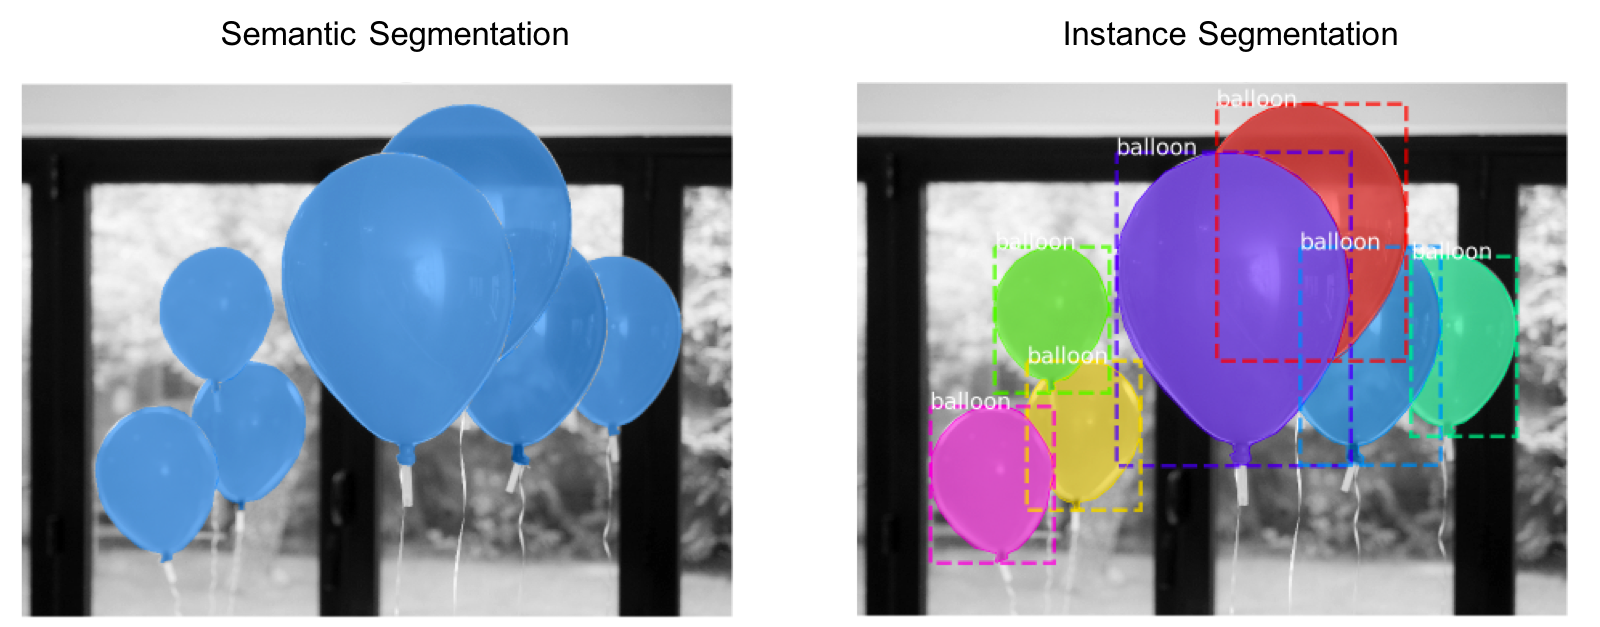
\includegraphics[width=15cm]{img/2_Theory/ss-is.png}
    \caption{Semantic Segmentation và Instance Segmentation}  
\end{center}
\end{figure}
\subsection{Kiến trúc hệ thống Image Segmentation}
\tab Kiến trúc cơ bản trong Image Segmentation bao gồm một bộ encoder (mã hoá) và decoder (giải mã).\\
\begin{figure}[!htb]
\begin{center}
    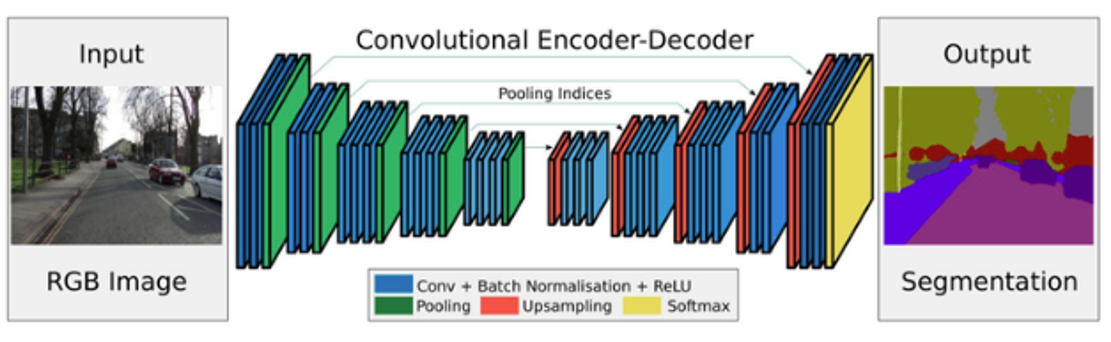
\includegraphics[width=15cm]{img/2_Theory/conv-encode-decode.png}
    \caption{Kiến trúc Convolutional Encoder-Decoder}  
\end{center}
\end{figure}\\
\tab Encoder trích xuất các tính năng từ hình ảnh thông qua các bộ lọc. Decoder chịu trách nhiệm tạo ra đầu ra cuối cùng thường là một mặt nạ phân đoạn chứa đường viền của đối tượng.
\subsection{Ứng dụng}
\tab Phân vùng ảnh có rất nhiều các ứng dụng trong y học, xe tự hành, xử lý ảnh vệ tinh, ...
\begin{itemize}
\item Y học: Trong y học, thuật toán Image Segmentation có thể hỗ trợ bác sĩ chẩn đoán khối u từ ảnh x-quang. Ưu điểm của Image Segmentation đó là không chỉ cho chúng ta biết vị trí của các khối u trong ảnh mà còn cho chúng ta biết được hình dạng của chúng.
\item Xe tự hành: Xe tự hành đòi hỏi phải liên tục nhận thức, xử lý và lên kế hoạch trong một môi trường luôn có sự thay đổi. Vì yêu cầu an toàn tuyệt đối và độ chính xác cao trong mọi quyết định nên một hệ thống xe tự hành cần phải xác định chính xác các vật thể xuất hiện khi tham gia giao thông như người, đèn tín hiệu, biển báo, vạch kẻ đường, xe cộ.
\item Xử lý ảnh vệ tinh: Các vệ tinh quay quanh trái đất sẽ liên tục thu thập hình ảnh bề mặt trái đất ở những vùng khác nhau. Từ các bức ảnh chụp vệ tinh, mô hình Image Segmentation sẽ phân đoạn hình ảnh thành tuyến đường, khu phố, biển cả, cây cối,….
\item Ứng dụng trong nông nghiệp: Chúng ta có thể tiết kiệm được một lượng lớn thuốc trừ sâu trong nông nghiệp nhờ sử dụng hệ thống phun thuốc trừ sâu tự động có khả năng phân biệt được diện tích cỏ và cây trồng dựa trên thuật toán Image Segmentation. Khi diện tích cỏ lấn át so với cây trồng thì hệ thống sẽ tự động kích hoạt.
\item Cảnh báo cháy rừng: Những hệ thống kiểm soát cháy rừng có thể segment được chính xác vị trí phát sinh các đám cháy từ ảnh chụp vệ tinh. Từ đó đưa ra cảnh báo về quy mô và mức độ lây lan của các đám cháy trên diện rộng.
\end{itemize}
\section{TwinLiteNet}
\tab Sau khi thực hiện nhiều thử nghiệm với các model khác nhau, nhóm đã quyết định sử dụng model TwinLiteNet\textsuperscript{\cite{twinlitenet}} cho đồ án. Khác biệt với các model nhận diện làn đường khác như UNet \textsuperscript{\cite{unet}}, LaneNet\textsuperscript{\cite{lanenet}}, YOLOPv2\textsuperscript{\cite{yolopv2}},... mà thường yêu cầu sử dụng nhiều tài nguyên và đòi hỏi phần cứng mạnh mẽ, TwinLiteNet được xây dựng như một model nhẹ (lightweight) nhưng vẫn đảm bảo độ chính xác và hiệu quả cao. Quyết định này nhằm tối ưu hiệu suất và độ nhẹ của model, giúp model có thể triển khai một cách linh hoạt trên các hệ thống có công suất tính toán hạn chế, như là những thiết bị nhúng trong xe tự hành.\\
\begin{figure}[h]
\begin{center}
    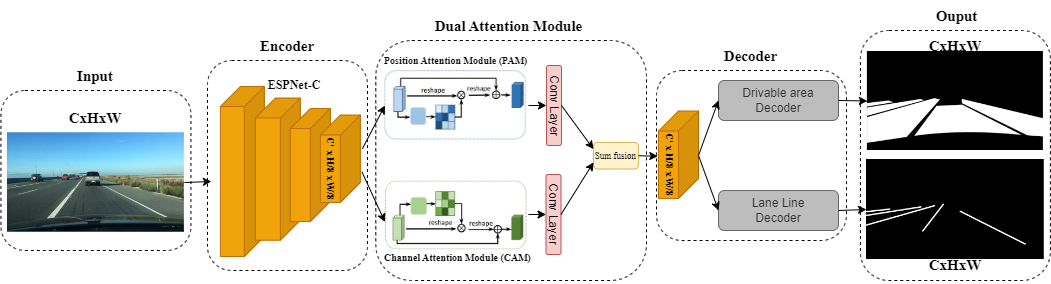
\includegraphics[width=16.5cm]{img/2_Theory/TwinLiteNet_arch.png}
    \caption{Kiến trúc TwinLiteNet}
\end{center}
\end{figure}\\
\tab TwinLiteNet sử dụng ESPNNet-C làm encoder để trích xuất các đặc trưng (feature) của ảnh gốc. Các đặc trưng được rút trích sẽ đi qua một bộ Dual Attention Module. Dual Attention Module bao gồm Position Attention Module (PAM) và Channel Attention Module (CAM). CAM tạo điều kiện thuận lợi cho việc tổng hợp thông tin đặc trưng của ảnh theo kênh, trong khi PAM được thiết kế để nắm bắt và tổng hợp các điểm ảnh (pixel) liên quan đến ngữ nghĩa trong miền không gian. Đầu ra của hai module sẽ được biến đổi bằng một lớp Convolutional và được tổng hợp lại bằng hàm cộng theo phần tử. Thay vì sử dụng một decoder duy nhất cho tất cả các loại đối tượng, thì TwinLiteNet sử dụng hai decoder để xử lý ma trận (map) đặc trưng và cho các tác vụ riêng biệt Drivable Area và Lane Segmentation
\subsection{Tập dữ liệu BDD100K}
\tab BDD100K\textsuperscript{\cite{bdd100k}} là tập dữ liệu hình ảnh dùng để huấn luyện các mô hình trí tuệ nhân tạo trong việc nhận dạng và phân loại hình ảnh. Tập dữ liệu này chứa hơn 100.000 hình ảnh và video được gắn nhãn, được thu thập từ các camera trên xe hơi. BDD100K được sử dụng rộng rãi trong các nghiên cứu về xe tự hành và các ứng dụng liên quan đến trí tuệ nhân tạo
\begin{figure}[!hbt]
\begin{center}
    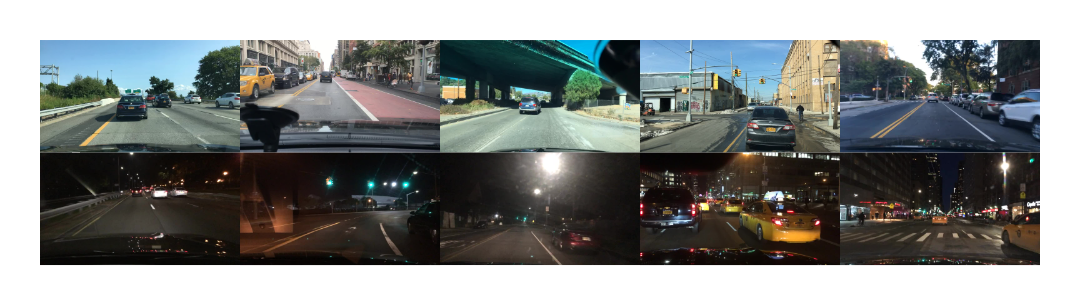
\includegraphics[width=16.5cm]{img/2_Theory/bdd100k.png}
    \caption{Minh hoạ tập dữ liệu BDD100K}
\end{center}
\end{figure}\\
\subsection{Hàm loss}
\tab Hai hàm loss được sử dụng trong model là Focal Loss\textsuperscript{\cite {focalloss}} và Tversky Loss\textsuperscript{\cite{tverskyloss}}. Focal Loss nhằm hạn chế sự ảnh hưởng của các mẫu dễ dự báo lên hàm loss và phạt nặng vào các mẫu khó dự báo, như ở phương trình. Ngược lại, Tversky Loss là một biến thể của Dice Loss, là độ đo để đánh giá kết quả segment. Khác với Dice Loss\textsuperscript{\cite{diceloss}}, Tversky Loss đánh thêm trọng số vào False Positives và False Negatives
\begin{equation}
Loss_{focal} = - \frac{1}{N}\sum_{C = 0}^{C - 1}\sum_{i = 1}^{N}p_i(c)(1 - \hat{p}_i(c))^{\gamma}log(\hat{p}_i(c))
\end{equation}
trong đó:
\begin{itemize}
    \item N: Số lượng pixel của ảnh
    \item C: Số lượng lớp, trong trường hợp này, một lớp là làn đường, và lớp còn lại là nền.
    \item \(\hat{p}_i(c)\): Xác định dự đoán cho pixel thứ 
i của lớp c
    \item \(p_i(c)\): Giá trị thực tế (ground truth) cho pixel thứ i của lớp c.
    \item \(\gamma\): Hệ số điều chỉnh cân bằng
\end{itemize}
\begin{equation}
Loss_{tversky} = - \frac{1}{N}(1 - \frac{TP(c)}{TP(c) - \alpha FN(c) \beta FP(c)})
\end{equation}
trong đó:
\begin{itemize}
    \item TP: True Positives
    \item FN: False Negatives
    \item FP: False Positives
    \item C: Số lượng lớp, trong trường hợp này, một lớp là làn đường, và lớp còn lại là nền.
    \item \(\alpha, \beta\): Điều khiển độ phạt cho FP và FN
\end{itemize}
Hàm loss tổng hợp sẽ có dạng:
\begin{equation}
Loss_{total} = Loss_{focal} + Loss_{tversky}
\end{equation}
\section{Bộ điều khiển PID}
\subsection{PID là gì}
\tab PID\textsuperscript{\cite{pid}} được viết tắt bởi cụm từ \textbf{Proportional Integral Derivative}, có nghĩa là 1 cơ chế phản hồi các vòng điều khiển, chúng được ứng dụng rộng rãi trong hệ thống điều khiển công nghiệp hiện đại.\\
\tab Bộ điều khiển này sử dụng nhiều trong những hệ thống điều khiển vòng kín có tín hiệu phản hồi. Nhiệm vụ của PID giúp tính toán giá trị sai số là hiệu số giữa giá trị đo thông số biến đổi với giá trị đặt mong muốn.\\
\begin{figure}[!hbt]
\begin{center}
    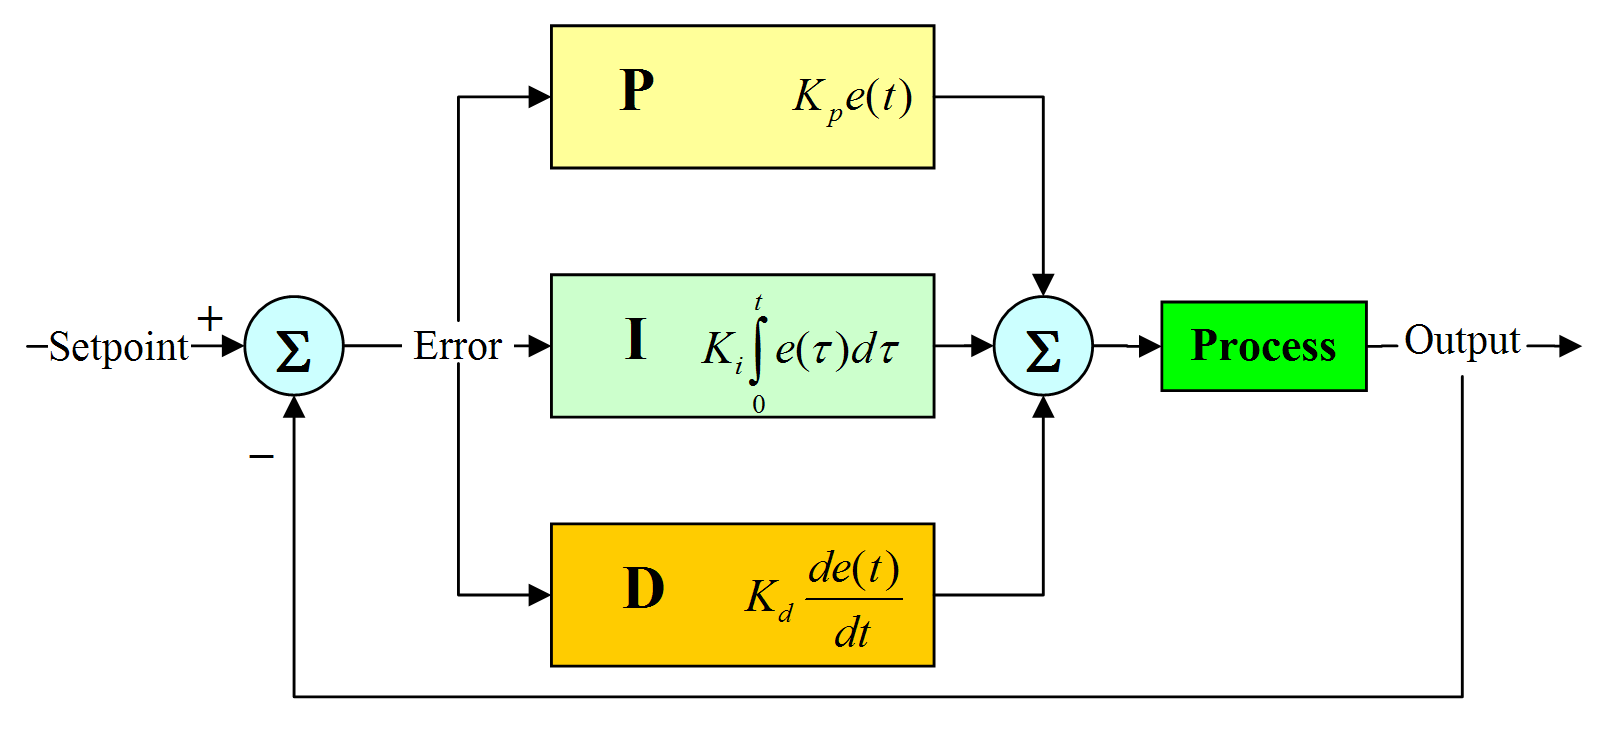
\includegraphics[width=14cm]{img/2_Theory/pid.png}
    \caption{Sơ đồ khối của hệ thống PID}
\end{center}
\end{figure}
\\
\tab Bộ thiết bị làm giảm tối đa sai số bằng cách điều chỉnh giá trị điều khiển đầu vào. Để đạt được hiệu quả mong muốn bởi thông số của PID cần phải thực hiện điều chỉnh theo tính chất hệ thống. Việc điều khiển sẽ giống nhau, còn thông số được phụ thuộc vào chính đặc thù của hệ thống đó.

\begin{itemize}
    \item P: là phương pháp điều chỉnh tỉ lệ, tạo ra tín hiệu điều chỉnh tỉ lệ với sai lệch đầu vào theo thời gian lấy mẫu.
    \item I: là tích phân của sai lệch theo thời gian lấy mẫu. Điều khiển tích phân là phương pháp điều chỉnh để tạo ra các tín hiệu điều chỉnh sao cho độ sai lệch giảm về 0. Từ đó cho biết tổng sai số tức thời theo thời gian hay sai số tích lũy trong quá khứ. Khi thời gian càng nhỏ thể hiện tác động điều chỉnh tích phân càng mạnh, tương ứng độ lệch càng nhỏ.
    \item D: là vi phân của sai lệch. Điều khiển vi phân tạo ra tín hiệu điều chỉnh sao cho tỉ lệ với tốc độ thay đổi sai lệch đầu vào. Thời gian càng lớn thì phạm vi điều chỉnh vi phân càng mạnh, tương ứng với bộ điều chỉnh đáp ứng với thay đổi đầu vào càng nhanh.
\end{itemize}
\subsection{Ứng dụng}
\tab Hiện nay PID được ứng dụng trong nhiều ngành nghề khác nhau:
\begin{itemize}
    \item Nó có thể được dùng để giảm các sai số, hạn chế sự dao động hay là giảm thời gian gian xác lập và độ vọt lố…
    \item Sử dụng để điều khiển mực nước: bộ điều khiển được tự động hóa nhờ vào các thiết bị điện tử như cảm biến, van điều khiển…
    \item Điều khiển biến tần: Các thiết bị điện tử kết hợp ở đây gồm có: van điều khiển lưu lượng, cảm biến nhiệt độ, biến tần điều khiển….
    \item Kiểm soát lưu lượng khí qua đường ống
\end{itemize}